\documentclass{article}

\usepackage{arxiv}

\usepackage[utf8]{inputenc} % allow utf-8 input
\usepackage[T1]{fontenc}    % use 8-bit T1 fonts
\usepackage{lmodern}        % https://github.com/rstudio/rticles/issues/343
\usepackage{hyperref}       % hyperlinks
\usepackage{url}            % simple URL typesetting
\usepackage{booktabs}       % professional-quality tables
\usepackage{amsfonts}       % blackboard math symbols
\usepackage{nicefrac}       % compact symbols for 1/2, etc.
\usepackage{microtype}      % microtypography
\usepackage{graphicx}

\title{spmodel: Spatial Modeling in \textbf{R} -- Supplementary Material}

\author{
    Michael Dumelle
    \thanks{Corresponding Author}
   \\
    United States \\
    Environmental Protection Agency \\
  200 SW 35th St, Corvallis, OR, 97333 \\
  \texttt{\href{mailto:Dumelle.Michael@epa.gov}{\nolinkurl{Dumelle.Michael@epa.gov}}} \\
   \And
    Matt Higham
   \\
    Department of Math, Computer Science, and Statistics \\
    St.~Lawrence University \\
  23 Romoda Drive, Canton, NY, 13617 \\
  \texttt{\href{mailto:mhigham@stlawu.edu}{\nolinkurl{mhigham@stlawu.edu}}} \\
   \And
    Jay M. Ver Hoef
   \\
    National Oceanic and Atmospheric Administration \\
    Alaska Fisheries Science Center \\
  Marine Mammal Laboratory, Seattle, WA, 98115 \\
  \texttt{\href{mailto:jay.verhoef@noaa.gov}{\nolinkurl{jay.verhoef@noaa.gov}}} \\
  }


% tightlist command for lists without linebreak
\providecommand{\tightlist}{%
  \setlength{\itemsep}{0pt}\setlength{\parskip}{0pt}}



\usepackage{amsmath,amsfonts,amssymb}
\usepackage{bm, bbm}
\usepackage{mathtools}
\mathtoolsset{showonlyrefs=true}
\begin{document}
\maketitle


\begin{abstract}
Enter the text of your abstract here.
\end{abstract}

\keywords{
    Spatial covariance
   \and
    Linear Model
   \and
    Autoregressive model
  }

\hypertarget{covariance-functions}{%
\section{Covariance Functions}\label{covariance-functions}}

\hypertarget{estimation}{%
\section{Estimation}\label{estimation}}

\hypertarget{likelihood-based-estimation}{%
\subsection{Likelihood-based
Estimation}\label{likelihood-based-estimation}}

Minus twice a profiled Gaussian log-likelihood, denoted
\(-2l(\bm{\theta} | \mathbf{y})\) is given by
\begin{equation}\label{eq:ml-lik}
  -2l(\bm{\theta} | \mathbf{y}) = \ln{|\mathbf{\Sigma}|} + (\mathbf{y} - \mathbf{X} \tilde{\bm{\beta}})^\intercal \mathbf{\Sigma}^{-1} (\mathbf{y} - \mathbf{X} \tilde{\bm{\beta}}) + n \ln{2\pi},
\end{equation} where
\(\tilde{\bm{\beta}} = (\mathbf{X}^\intercal \mathbf{\Sigma}^{-1} \mathbf{X})^{-1} \mathbf{X}^\intercal \mathbf{\Sigma}^{-1} \mathbf{y}\).
Minimizing Equation\(~\)\ref{eq:ml-lik} yields
\(\bm{\hat{\theta}}_{ml}\), the maximum likelihood estimates for
\(\bm{\theta}\). Then a closed for solution exists for
\(\bm{\hat{\beta}}_{ml}\), the maximum likelihood estimates for
\(\bm{\beta}\): \(\bm{\hat{\beta}}_{ml} = \tilde{\bm{\beta}}_{ml}\),
where \(\tilde{\bm{\beta}}_{ml}\) is \(\tilde{\bm{\beta}}\) evaluated at
\(\bm{\hat{\theta}}_{ml}\). Unfortunately \(\bm{\hat{\theta}}_{ml}\) can
be badly biased for \(\bm{\theta}\) (especially for small sample sizes),
which impacts the estimation of \(\bm{\beta}\) (Patterson and Thompson
1971). This bias occurs due to the simultaneous estimation of
\(\bm{\beta}\) and \(\bm{\theta}\) To reduce this bias, restricted
maximum likelihood estimation (REML) emerged (Patterson and Thompson
1971; Harville 1977; Wolfinger, Tobias, and Sall 1994). It can be shown
that integrating \(\bm{\beta}\) out of a Gaussian likelihood yields the
restricted Gaussian likelihood used in REML estimation. Minus twice a
restricted Gaussian log-likelihood, denoted
\(-2l_R(\bm{\theta} | \mathbf{y})\) is given by
\begin{equation}\label{eq:reml-lik}
  -2l_R(\bm{\theta} | \mathbf{y}) = -2l(\bm{\theta} | \mathbf{y})  + \ln{|\mathbf{X}^\intercal \mathbf{\Sigma}^{-1} \mathbf{X}|} - p \ln{2\pi} ,
\end{equation} where \(p\) equals the dimension of \(\bm{\beta}\).
Minimizing Equation\(~\)\ref{eq:reml-lik} yields
\(\bm{\hat{\theta}}_{reml}\), the restricted maximum likelihood
estimates for \(\bm{\theta}\). Then a closed for solution exists for
\(\bm{\hat{\beta}}_{reml}\), the restricted maximum likelihood estimates
for \(\bm{\beta}\):
\(\bm{\hat{\beta}}_{reml} = \tilde{\bm{\beta}}_{reml}\), where
\(\tilde{\bm{\beta}}_{reml}\) is \(\tilde{\bm{\beta}}\) evaluated at
\(\bm{\hat{\theta}}_{reml}\).

Generally the overall variance, \(\sigma^2\), can be profiled out of
Equation\(~\)\ref{eq:ml-lik} and Equation\(~\)\ref{eq:reml-lik}. This
reduces the number of parameters requiring optimization by one, which
can dramatically reduce estimation time. For example, profiling
\(\sigma^2\) out of Equation\(~\)\ref{eq:ml-lik} yields
\begin{equation}\label{eq:ml-plik}
  -2l^*(\bm{\theta}^* | \mathbf{y}) = \ln{|\mathbf{\Sigma^*}|} + n\ln[(\mathbf{y} - \mathbf{X} \tilde{\bm{\beta}})^\intercal \mathbf{\Sigma}^{-1} (\mathbf{y} - \mathbf{X} \tilde{\bm{\beta}})] + n + n\ln{2\pi / n}.
\end{equation} After finding \(\hat{\bm{\theta}}^*_{ml}\) a closed form
solution for \(\hat{\sigma}^2_{ml}\) exists:
\(\hat{\sigma}^2_{ml} = [(\mathbf{y} - \mathbf{X} \bm{\tilde{\beta}})^\intercal \mathbf{\Sigma}^{-1} (\mathbf{y} - \mathbf{X} \tilde{\bm{\beta}})] / n\).
Then \(\bm{\hat{\theta}}^*_{ml}\) is combined with
\(\hat{\sigma}^2_{ml}\) to yield \(\bm{\hat{\theta}}_{ml}\) and
subsequently \(\bm{\hat{\beta}}_{ml}\). A similar result holds for REML
estimation. Profiling \(\sigma^2\) out of Equation\(~\)\ref{eq:reml-lik}
yields \begin{equation}\label{eq:reml-plik}
  -2l_R^*(\bm{\theta}^* | \mathbf{y}) = \ln{|\mathbf{\Sigma^*}|} + (n - p)\ln[(\mathbf{y} - \mathbf{X} \tilde{\bm{\beta}})^\intercal \mathbf{\Sigma}^{-1} (\mathbf{y} - \mathbf{X} \tilde{\bm{\beta}})] + (n - p) + (n - p)\ln2\pi / (n - p).
\end{equation} After finding \(\hat{\bm{\theta}}^*_{reml}\) a closed
form solution for \(\hat{\sigma}^2_{reml}\) exists:
\(\hat{\sigma}^2_{reml} = [(\mathbf{y} - \mathbf{X} \bm{\tilde{\beta}})^\intercal \mathbf{\Sigma}^{-1} (\mathbf{y} - \mathbf{X} \tilde{\bm{\beta}})] / (n - p)\).
Then \(\bm{\hat{\theta}}^*_{reml}\) is combined with
\(\hat{\sigma}^2_{reml}\) to yield \(\bm{\hat{\theta}}_{reml}\) and
subsequently \(\bm{\hat{\beta}}_{reml}\).

Both ML and REML estimation rely on the an \(n \times n\) covariance
matrix inverse. Inverting an \(n \times n\) matrix is an enormous
computational demand that scales cubically with the sample size. For
this reason, ML and REML have historically been unfeasible to implement
in their standard form with data larger than a few thousand
observations. This motivates the use for the big data approaches
outlined in Section\(~\)(INSERT SECTION).

It is worth noting that the inverses themselves are not strictly needed
for estimation (or prediction), though at least their square root is
needed. In spmodel, calculating this square root requires a Cholesky
decomposition, which still scales cubically with the sample size.
Computing the Cholesky decomposition, however, is far more
computationally efficient than computing the inverse. To see why only
the Cholesky decomposition is needed, recall that the Cholesky
decomposition of the covariance matrix \(\mathbf{\Sigma}\) is
\(\mathbf{C}\mathbf{C}^\intercal\), where \(\mathbf{C}\) is a lower
triangular matrix (so
\(\mathbf{C}\mathbf{C}^\intercal = \mathbf{\Sigma}\)). In the ML and
REML likelihoods, \(\mathbf{\Sigma}^{-1}\) is not needed on its own,
only \(\mathbf{X}^\intercal \mathbf{\Sigma}^{-1} \mathbf{X}\) and
\(\mathbf{X}^\intercal \mathbf{\Sigma}^{-1} \mathbf{y}\) are needed. We
can rewrite the \(\mathbf{X}^\intercal \mathbf{\Sigma}^{-1} \mathbf{X}\)
as
\(\mathbf{X}^\intercal (\mathbf{C}^\intercal)^{-1} \mathbf{C}^{-1} \mathbf{X} = (\mathbf{C}^{-1} \mathbf{X})^\intercal \mathbf{C}^{-1} \mathbf{X}\).
Then \(\mathbf{C}^{-1} \mathbf{X}\) is efficiently solved by noticing
that \(\mathbf{C}^{-1} \mathbf{X} = \mathbf{A}\) for some matrix
\(\mathbf{A}\) implies \(\mathbf{X} = \mathbf{C} \mathbf{A}\). This
system can be efficiently solved for \(\mathbf{A}\) using linear forward
solves (forward substitution). Then
\(\mathbf{X}^\intercal \mathbf{\Sigma}^{-1} \mathbf{X} = \mathbf{A}^\intercal \mathbf{A}\).
A similar approach is used to solve
\(\mathbf{X}^\intercal \mathbf{\Sigma}^{-1} \mathbf{y}\). Still, using
Cholesky decomositions is unfeasible for sample sizes larger than a few
thousand observations.

\hypertarget{semivariogram-based-estimation}{%
\subsection{Semivariogram-based
Estimation}\label{semivariogram-based-estimation}}

An alternative approach to likelihood-based estimation is
semivariogram-based estimation. The semivariogram of a constant-mean
process \(\mathbf{y}\) is the expectation of the squared half-difference
between two observations \(h\) distance units apart. More formally, the
semivariogram is denoted \(\gamma(h)\) and defined as
\begin{equation}\label{eq:sv}
  \gamma(h) = \text{E}(y_i - y_j)^2 / 2 ,
\end{equation} where \(||y_i - y_j||_2 = h\) (the Euclidean distance).
When the process \(\mathbf{y}\) is second-order stationary, the
semivariogram and covariance function are intimately connected:
\(\gamma(h) = \text{Cov}(0) - \text{Cov}(h)\), where \(\text{Cov}(0)\)
is the covariance function evaluated at 0 (which is the overall
variance, \(\sigma^2\)) and \(\text{Cov}(h)\)is the covariance function
evaluated at \(h\). Both semivariogram approaches described next are
more computationally efficient than ML or REML because their major
computational burden (calculations based on pairs) scale the squared
sample size (i.e., not the cubed sample size).

\hypertarget{weighted-least-squares}{%
\subsubsection{Weighted Least Squares}\label{weighted-least-squares}}

The empirical semivariogram is a moment-based estimate of the
semivariogram denoted by \(\hat{\gamma}(h)\) and defined as
\begin{equation}\label{eq:esv}
  \hat{\gamma}(h) = \frac{1}{2|N(h)|} \sum_{N(h)} (y_i - y_j)^2, 
\end{equation} where \(N(h)\) is the set of observations in
\(\mathbf{y}\) that are \(h\) units apart (distance classes) and
\(|N(h)|\) is the cardinality of \(N(h)\) (Cressie 1993). Often the set
\(N(h)\) contains observations that are \(h \pm \alpha\) apart -- this
approach is known as ``binning'' the empirical semivariogram. Typically,
only certain \(h\) considered when constructing
Equation\(~\)\ref{eq:esv} -- a commonly used cutoff is to ignore \(h\)
larger than half the maximum distance in the domain. One criticism of
the empirical semivariogram is that distance bins and cutoffs tend to be
artitrarily chosen (i.e., not chosen according to some statistical
criteria).

Equation\(~\)\eqref{eq:esv} is viewed as the average squared
half-distance between two observations in \(\mathbf{y}\). Cressie (1985)
proposed estimating \(\bm{\theta}\) by minimizing an objective function
that involves \(\gamma{h}\) and \(\hat{\gamma}(h)\) and is based on a
weighted least squares criterion. This criterion is defined as
\begin{equation}\label{eq:svwls}
  \sum_i w_i [\hat{\gamma}(h)_i - \gamma(h)_i]^2,
\end{equation} where \(w_i\), \(\hat{\gamma}(h)_i\), and \(\gamma(h)_i\)
are the weights, empirical semivariogram, and semivariogram for the
\(i\)th distance class. Minimizing Equation\(~\)\eqref{eq:svwls} yields
\(\bm{\hat{\theta}}_{wls}\), the semivariogram weighted least squares
estimates of \(\bm{\theta}\). After estimating \(\bm{\theta}\),
\(\bm{\beta}\) estimates are constructed using (empirical) generalized
least squares:
\(\bm{\hat{\beta}}_{wls} = (\mathbf{X}^\intercal \hat{\mathbf{\Sigma}}^{-1} \mathbf{X})^{-1} \mathbf{X}^\intercal \hat{\mathbf{\Sigma}}^{-1} \mathbf{y}\),
where \(\hat{\mathbf{\Sigma}}^{-1}\) is \(\mathbf{\Sigma}\) evaluated at
\(\bm{\hat{\theta}}_{wls}\).

Cressie (1985) recommends setting the \(w_i\) in
Equation\(~\)\eqref{eq:svwls} as \(w_i = |N(h)| / \gamma(h)_i^2\), which
gives more weights to distance classes with more observations
(\(|N(h)|\)) and semivariances at shorter distances
(\(1 / \gamma(h)_i^2\)). The default in spmodel is to use these \(w_i\)
-- the type of \(w_i\) is changed via the \texttt{weights} argument to
\texttt{splm()}. Table\(~\)\ref{tab:weights} contains all \(w_i\)
available in spmodel.

\begin{table}\label{tab:weights}
  \centering
  \begin{tabular}{c|c|c}
  \hline
  $w_i$ Name & $w_i$ Form & \texttt{weight = } \\
  Cressie & $|N(h)| / \gamma(h)_i^2$ & \texttt{"cressie"} \\
  Cressie (Denominator) Root & $|N(h)| / \gamma(h)_i$ & \texttt{"cressie-droot"} \\
  Cressie No Pairs & $1 / \gamma(h)_i^2$ & \texttt{"cressie-nopairs"} \\
  Cressie (Denominator) Root No Pairs & $1 / \gamma(h)_i$ & \texttt{"cressie-droot-nopairs"} \\
  Pairs & $|N(h)|$ & \texttt{"pairs"} \\
  Pairs Inverse Distance & $|N(h)| / h^2$ & \texttt{"pairs-invd"} \\
  Pairs Inverse (Root) Distance & $|N(h)| / h$ & \texttt{"pairs-invsd"} \\
  Ordinary Least Squares & 1 & \texttt{ols}
  \end{tabular}
  \caption{spmodel table weights}
\end{table}

Additionally, the number of \(N(h)\) classes and maximum distance for
\(h\) are specified by passing the \texttt{bins} and \texttt{cutoff}
arguments to \texttt{splm()} (these arguments are passed via
\texttt{...} to \texttt{esv()}). The default value for \texttt{bins} is
15 and the default value for the maximum \(h\) is half the maximum
distance of the spatial domain's bounding box.

Recall that the semivariogram is defined for a constant-mean process.
Generally, \(\mathbf{y}\) does not necessarily have a constant mean. So
the empirical semivariogram and \(\bm{\hat{\theta}}_{wls}\) are
typically constructed using the residuals from an ordinary least squares
regression of \(\mathbf{y}\) on \(\mathbf{X}\) -- these residuals are
assumed to have mean zero.

After

\hypertarget{composite-likelihood}{%
\subsubsection{Composite Likelihood}\label{composite-likelihood}}

The composite likelihood approach involves constructing a likelihood
based on conditional or marginal events for which log-likelihoods are
available and then adding together these individual components.
Composite likelihoods are attractive because they behave very similar to
likelihoods but are easier to handle, both from a theoretical and a
computational perspective. Curriero and Lele (1999) derive a particular
composite likelihood for estimating semivariogram parameters. The
negative log of this composite likelihood, denoted \(\text{CL}(h)\), is
given by \begin{equation}\label{eq:svcl}
  \text{CL}(h) = \sum_{i = 1}^{n - 1} \sum_{j > i} \left( \frac{(y_i - y_j)^2}{2\gamma(h)} + \ln(\gamma(h)) \right)
\end{equation} where \(\gamma(h)\) is the semivariogram (that depends on
parameter vector \(\bm{\theta}\)). Minimizing Equation\(~\)\ref{eq:svcl}
yields \(\bm{\hat{\theta}}_{cl}\), the semivariogram composite
likelihood estimates of \(\bm{\theta}\). After estimating
\(\bm{\theta}\), \(\bm{\beta}\) estimates are constructed using
(empirical) generalized least squares:
\(\bm{\hat{\beta}}_{cl} = (\mathbf{X}^\intercal \hat{\mathbf{\Sigma}}^{-1} \mathbf{X})^{-1} \mathbf{X}^\intercal \hat{\mathbf{\Sigma}}^{-1} \mathbf{y}\),
where \(\hat{\mathbf{\Sigma}}^{-1}\) is \(\mathbf{\Sigma}\) evaluated at
\(\bm{\hat{\theta}}_{cl}\).

An advantage of the composite likelihood approach to semivariogram
estimation is that it does not require arbitrarily specifying empircial
semivariogram bins and cutoffs. It does tend to be more computationally
demanding than the weighted least squares, however, as the composite
likelihood is constructed from \(\binom{n}{2}\) pairs for a sample size
\(n\), whereas the weighted least squares approach only requires
calculating \(\binom{|N(h)|}{2}\) pairs for each distance bin \(N(h)\).
As with the weighted least squares approach, Equation\(~\)\ref{eq:svcl}
requires constant-mean process, so typically the residuals from an
ordinary least squares regression of \(\mathbf{y}\) on \(\mathbf{X}\)
are used to estimate \(\bm{\theta}\).

\hypertarget{hypothesis-testing}{%
\section{Hypothesis Testing}\label{hypothesis-testing}}

\hypertarget{the-general-linear-hypothesis-test}{%
\subsection{The General Linear Hypothesis
Test}\label{the-general-linear-hypothesis-test}}

Hypothesis tests for each element in \(\hat{\bm{\beta}}\) are available
in \texttt{summary()}.

\begin{verbatim}

Call:
splm(formula = y ~ x + group, data = exdata, spcov_type = "exponential", 
    xcoord = xcoord, ycoord = ycoord)

Residuals:
     Min       1Q   Median       3Q      Max 
-1.91090 -0.38965  0.07808  0.56560  2.29718 

Coefficients (fixed):
            Estimate Std. Error z value Pr(>|z|)  
(Intercept) -0.65261    0.38911  -1.677   0.0935 .
x           -0.07809    0.07357  -1.061   0.2885  
group2       0.29110    0.20997   1.386   0.1656  
group3       0.37734    0.20857   1.809   0.0704 .
group4       0.32637    0.21531   1.516   0.1296  
---
Signif. codes:  0 '***' 0.001 '**' 0.01 '*' 0.05 '.' 0.1 ' ' 1

Pseudo R-squared: 0.04864

Coefficients (spatial covariance):
    de     ie  range 
0.6330 0.3791 1.2350 

Spatial covariance type: exponential
\end{verbatim}

Test statistics are the ratio of the estimate to its standard error.
These tests are useful for continuous predictors, but for categorical
predictors, \texttt{summary()} only provides test statistics for each
level, not all levels simultaneously. To find a test statistic for a
categorical variable, there are two approaches. The first is to use
\texttt{anova()}.

\begin{verbatim}
Analysis of Variance Table

Response: y
                Df     X2 Pr(>X2)
(Intercept) 1.0000 2.8129  0.0935
x           1.0000 1.1267  0.2885
group       3.0000 3.8742  0.2754
\end{verbatim}

Test statistics from \texttt{anova()} are formed using the general
linear hypothesis test. Let \(\mathbf{L}\) be an \(l \times p\) contrast
matrix and \(l_0\) be an \(l \times 1\) vector. The null hypothesis is
that \(\mathbf{L} \bm{\hat{\beta}} = l_0\) and the alternative
hypothesis is that \(\mathbf{L} \bm{\hat{\beta}} \neq l_0\). Usually,
\(l_0\) is the zero vector (and in spmodel, this is assumed). The test
statistic, denoted \(X^2\), is given by \begin{equation}\label{eq:glht}
  \tilde{F} = [(\mathbf{L} \bm{\hat{\beta}} - l_0)^\intercal(\mathbf{L} (\mathbf{X}^\intercal \mathbf{\hat{\Sigma}} \mathbf{X})^{-1} \mathbf{L}^\intercal)^{-1}(\mathbf{L} \bm{\hat{\beta}} - l_0)]/ rank(\mathbf{L})
\end{equation} By default, \(\mathbf{L}\) is chosen such that each
variable in the data used to fit the model is tested. If this deafult is
not desired, the \texttt{Terms} and \texttt{L} arguments can be used to
pass user-defined \(\mathbf{L}\) matrices to \texttt{anova()}.

It is notoriously difficult to determine appropriate p-values for linear
mixed models based on the general linear hypothesis test. lme4, for
example, does not report p-values by default. There are three reasons we
focus on next that explain why obtaining p-values is so challenging.

\begin{itemize}
\tightlist
\item
  The first (and often most important) challenge is that when estimating
  \(\bm{\theta}\), it is usually not clear what the null distribution of
  \(\tilde{F}\). In certain cases such as ordinary least squares
  regression or certain experimental designs (e.g., blocked design,
  split plot design, etc.), \(\tilde{F}\) is F-distributed with known
  numerator and denominator degrees of freedom. But outside of these
  well-studied cases, no general results exist.
\item
  The second challenge is that the standard error of \(\tilde{F}\) does
  not account for the uncertainty in \(\bm{\hat{\theta}}\). For some
  approaches to addressing this problem, see Kackar and Harville (1984),
  Prasad and Rao (1990), Harville and Jeske (1992), and Kenward and
  Roger (1997).
\item
  The third challenge is in determining denominator degrees of freedom.
  Again, in certain cases, these are known -- but this is not true in
  general. For some approaches to addressing this problem, see
  Satterthwaite (1946), Schluchter and Elashoff (1990), Hrong-Tai Fai
  and Cornelius (1996), Kenward and Roger (1997), Littell et al. (2006),
  Pinheiro and Bates (2006), and Kenward and Roger (2009).
\end{itemize}

For these reasons, spmodel assumes a large-sample, Chi-squared
approximation when calculating p-values. This approach addresses the
three points above by assuming that with a large enough sample size:

\begin{itemize}
\tightlist
\item
  The numerator of \(\tilde{F}\) tends to be asymptotically Chi-squared
  (under certain conditions) with \(rank(\mathbf{L})\) degrees of
  freedom.
\item
  The uncertainty from estimating \(\bm{\hat{\theta}}\) is small enough
  to be safely ignored.
\end{itemize}

Because the approximation is asymptotic, degree of freedom adjustments
can be ignored (it is also worth noting that an F distribution with
infinite denominator degrees of freedom is a scaled (by \(rank{L}\))
Chi-squared distribution). A takeaway here is that this asymptotic
approximation implies these p-values are likely unreliable with small
samples.

A second approach to determining p-values is a likelihood ratio test for
nested models. Let
\(l(\bm{\hat{\theta}}_0, \bm{\hat{\beta}}_0 | \mathbf{y} )\) be the
log-likelihood from some reduced model and
\(l(\bm{\hat{\theta}}_1, \bm{\hat{\beta}}_1 | \mathbf{y} )\) be the
log-likelihood from some full model. When the reduced model is nested in
the full model (i.e., the reduced model can be obtained by fixing some
parameters of the full model),
\([-2l(\bm{\hat{\theta}}_0, \bm{\hat{\beta}}_0 | \mathbf{y} )] - [-2l(\bm{\hat{\theta}}_1, \bm{\hat{\beta}}_1 | \mathbf{y} )]\)
is asymptotically Chi-squared with degrees of freedom equal to the
difference in estimated parameters between the full and reduced model.
To see whether there is evidence of spatial covariance, run

\begin{verbatim}
Likelihood Ratio Test

Response: y
           Df     X2 Pr(>X2)
1 vs 2  2.000 20.139       0
\end{verbatim}

This output suggests evidence of spatial covariance. Because the
likelihood relies on minimized likelihoods, they are only defined for ML
or REML estimation. Furthermore, for REML estimation, likelihood ratio
tests can only be used to compare nested models whose fixed effect
structure does not change. This is because the REML likelihood
\eqref{eq:reml-lik} depends on the fixed effects through
\(\ln{|\mathbf{X}^\intercal \mathbf{\Sigma}^{-1} \mathbf{X}|}\). To use
likelihood ratio tests for assessing the importance of fixed effects,
parameters must be estimated using ML. When using likelihood ratio tests
to assess the importance of parameters on the boundary of a parameter
space (e.g., a variance parameter being zero), p-values tend to be too
large (Self and Liang 1987; Stram and Lee 1994; Goldman, Whelan, and
Simon 2000; Pinheiro and Bates 2006).

\hypertarget{random-effects}{%
\section{Random Effects}\label{random-effects}}

\hypertarget{blups}{%
\subsection{BLUPs}\label{blups}}

\hypertarget{prediction}{%
\section{Prediction}\label{prediction}}

Predictions are often the primary goal of a data analysis. spmodel
performs best linear unbiased prediction, which is equivalent to
Kriging, using the \texttt{predict()} function. Let \(\mathbf{y}_o\) be
a vector of observed variables and \(\mathbf{y}_u\) be a vector of
unobserved variables. Let \(\mathbf{X}_o\) and \(\mathbf{X}_u\) be the
fixed effect design matrices of \(\mathbf{y}_o\) and \(\mathbf{y}_u\),
respectively. Let \(\mathbf{\Sigma}_o\) and \(\mathbf{\Sigma}_u\) be the
covariance matrices of \(\mathbf{y}_o\) and \(\mathbf{y}_u\),
respectively. The (empirical) best linear unbiased predictor (BLUP;
Kriging predictor) of \(\mathbf{y}_u\), denoted \(\mathbf{\dot{y}_u}\)
is given by \begin{equation}\label{eq:blup}
  \mathbf{\dot{y}_u} =  \mathbf{X}_u \bm{\hat{\beta}} + \mathbf{\hat{c}}_{uo} \mathbf{\hat{\Sigma}}^{-1}_o (\mathbf{y}_o - \mathbf{X}_o \bm{\hat{\beta}}) ,
\end{equation} where
\(\mathbf{\hat{c}}_{uo} = \hat{\text{Cov}}(\mathbf{y}_u, \mathbf{y}_o)\)
and
\(\bm{\hat{\beta}} = (\mathbf{X}^\intercal \mathbf{\hat{\Sigma}}^{-1} \mathbf{X})^{-1}\).
One can show that \(\hat{\text{Cov}}(\mathbf{\dot{y}})\) is
\begin{equation}\label{eq:vblup}
  \text{Cov}(\mathbf{\dot{y}}) = \mathbf{\hat{\Sigma}}_u - \mathbf{\hat{c}}_{uo} \mathbf{\hat{\Sigma}}^{-1}_o \mathbf{\hat{c}}_{uo}^\intercal + \mathbf{H}(\mathbf{X}^\intercal \mathbf{\hat{\Sigma}}^{-1} \mathbf{X})^{-1}\mathbf{H}^\intercal ,
\end{equation} where
\(\mathbf{H} = (\mathbf{X}_u - \mathbf{\hat{c}}_{uo} \mathbf{\hat{\Sigma}}^{-1}_o \mathbf{X}_o)\).
When \(\texttt{predict(..., interval = "none")}\), predictions are
obtained using Equation\(~\)\ref{eq:blup}. If \texttt{se.fit = TRUE},
standard errors are the square root of the diagonal of
Equation\(~\)\ref{eq:vblup}. When
\texttt{predict(..., interval = "prediction")}, predictions are obtained
using Equation\(~\)\ref{eq:blup} and standard errors used for the lower
and upper bound of the prediction intervals are obtained via the square
root of the diagonal of Equation\(~\)\ref{eq:vblup} (these are also what
are returned if \texttt{se.fit = TRUE}). When
\texttt{predict(..., interval = "confidence")}, mean estimates are
obtained using \(\mathbf{X}_u \bm{\hat{\beta}}\) and standard errors
used for the lower and upper bound of the confidence intervals are
obtained via the square root of the diagonal of
\((\mathbf{X}^\intercal \mathbf{\hat{\Sigma}}^{-1} \mathbf{X})^{-1}\)
(these are also what are returned if \texttt{se.fit = TRUE}).

For autoregressive models, an extra step is required to obtain
\(\hat{\Sigma}^{-1}_o\) and \(\hat{\Sigma}^{-1}_u\), as they depend on
one another through the locations of \(\mathbf{y}_o\) and
\(\mathbf{y}_u\). Let \(\hat{\Sigma}^{-1}\) be the inverse covariance
matrix of \(\mathbf{y}_o\) and \(\mathbf{y}_u\) (which we directly
specify for autoregressive models). If the data are small enough, then
\(\hat{\Sigma}^{-1}\) can be inverted, yielding \(\hat{\Sigma}\). Then
appropriate subsets can then used to obtain the components needed for
prediction. A faster way to obtain relevant components required for
prediction does exist and is worth mentioning -- \(\hat{\Sigma}^{-1}\)
can be represented blockwise as \begin{equation}\label{eq:auto_hw}
  \hat{\Sigma}^{-1} =
  \begin{bmatrix}
    \mathbf{\hat{\Sigma}}^{*}_{o, o} & \mathbf{\hat{\Sigma}}^{*}_{o, u} \\
    \mathbf{\hat{\Sigma}}^{*}_{u, o} & \mathbf{\hat{\Sigma}}^{*}_{u, u}
  \end{bmatrix},
\end{equation} where the dimensions of the blocks are indexed by the
matrix subscripts (rows then columns). All of the terms required for
prediction can be obtained from this block representation. Wolf (1978)
shows that \begin{equation}\label{eq:hw_forms}
  \begin{split}
    \hat{\Sigma}^{-1}_o & = \mathbf{\hat{\Sigma}}^{*}_{o, o} - \mathbf{\hat{\Sigma}}^{*}_{o, u} (\mathbf{\hat{\Sigma}}^{*}_{u, u})^{-1} \mathbf{\hat{\Sigma}}^{*}_{u, o} \\
    \hat{\Sigma}_u & = (\mathbf{\hat{\Sigma}}^{*}_{u, u} - \mathbf{\hat{\Sigma}}^{*}_{u, o} (\mathbf{\hat{\Sigma}}^{*}_{o, o})^{-1} \mathbf{\hat{\Sigma}}^{*}_{o, u})^{-1} \\
    \text{Cov}(\mathbf{y}_o, \mathbf{y}_u) & = - \hat{\Sigma}_o \mathbf{\hat{\Sigma}}^{*}_{o, u} (\mathbf{\hat{\Sigma}}^{*}_{u, u})^{-1}
  \end{split}
\end{equation} A similar result exists for the log determinant (used in
ML and REML estimation).

\hypertarget{geometric-anisotropy}{%
\section{(Geometric) Anisotropy}\label{geometric-anisotropy}}

A spatial process is geometrically isotropic if its covariance decays
equally in all directions. A spatial process is geometrically
anisotropic if its covariance does not decay equally in all directions
(i.e., is not isotropic). Let \(h\) represent distance, \(\alpha\)
represent an angle in \([0, \pi]\), and \(\tau\) represent a scaling
factor in \([0, 1]\). Geometric anisotropy is accommodate through a
specific rotation and scaling of the x-coordinate and y-coordinate. Then
a new distance, \(h*\), corresponds to an isotropic process. The scaling
works by rotating the major axis of the covariance clockwise onto a
transformed x-axis and scaling the minor axis of the covariance along
the transformed y-axis. Geometrically, this transformation and
re-scaling is achieved via \begin{equation}
  \begin{bmatrix}
    \mathbf{x}^* \\
    \mathbf{y}^*
  \end{bmatrix} = 
  \begin{bmatrix}
    1 & 0 \\
    0 & 1 / \tau
  \end{bmatrix}
  \begin{bmatrix}
    \cos(\alpha) & \sin(\alpha) \\
    -\sin(\alpha) & \cos(\alpha)
  \end{bmatrix}  
  \begin{bmatrix}
    \mathbf{x} \\
    \mathbf{y}
  \end{bmatrix}
\end{equation}

Then covariance parameters are estimated using the transformed
coordinates to compute distances. An anisotropy transformation is
visualized in Figure\(~\)\ref{fig:anisotropy}.

\begin{figure}
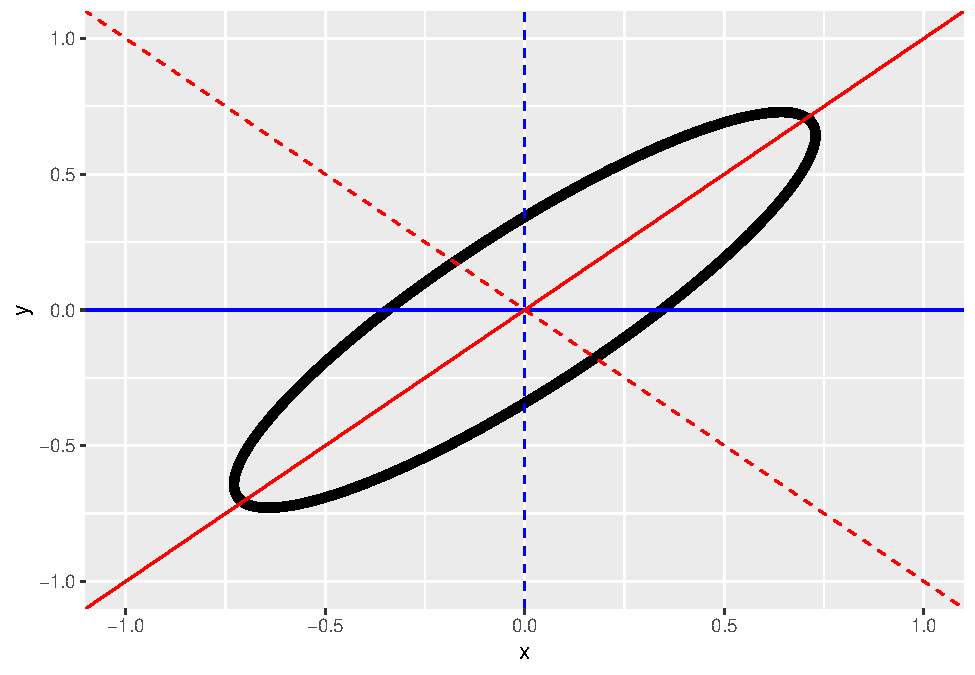
\includegraphics[width=0.33\linewidth]{supplementary_files/figure-latex/anisotropy-1} 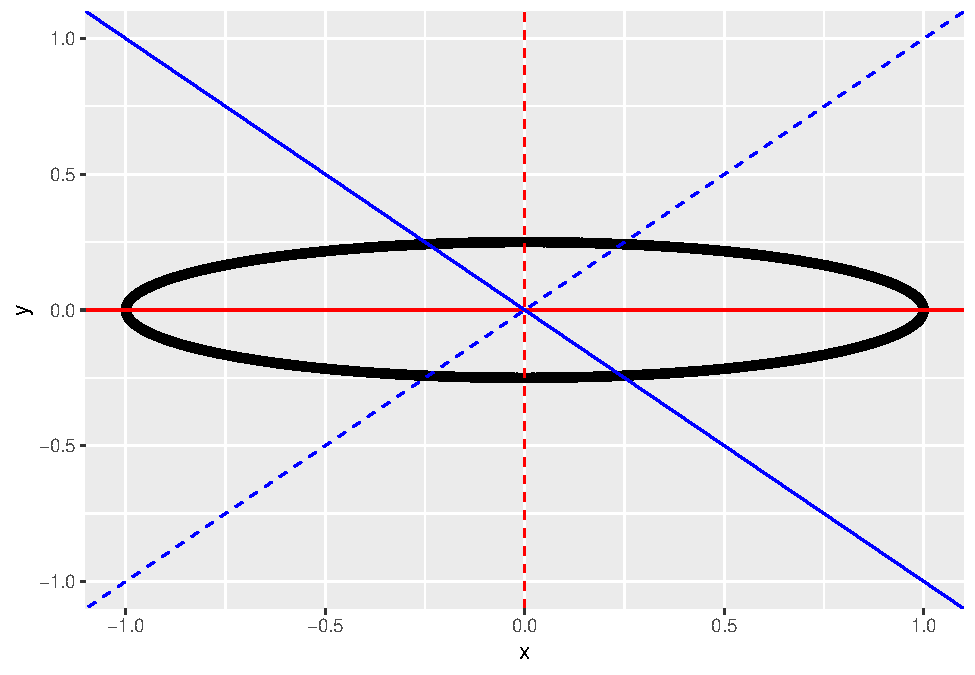
\includegraphics[width=0.33\linewidth]{supplementary_files/figure-latex/anisotropy-2} 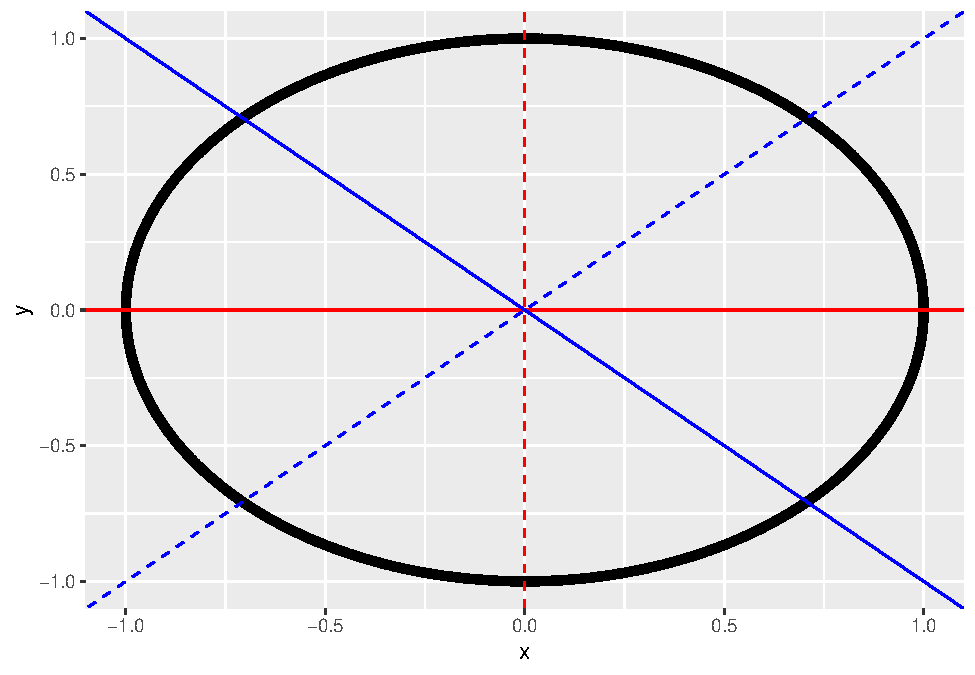
\includegraphics[width=0.33\linewidth]{supplementary_files/figure-latex/anisotropy-3} \caption{In the first figure, the ellipse of an anisotropy covariance is shown. In the second figure, the ellipse is rotated so the major axis is the transformed x-axis and the minor axis is the transformed y-axis. In the third figure, the ellipse is scaled so the ellipse becomes a circle. Then covariance estimation can be performed (using the transformed coordinates that compose the third figure).}\label{fig:anisotropy}
\end{figure}

In spmodel, anisotropy parameters (\(\alpha\) and \(\tau\)) can be
estimated using ML or REML by setting the \texttt{anisotropy} argument
to \texttt{TRUE} or by specifying one of the anisotropy parameters as
unknown or known and different from zero in \texttt{spcov\_initial}.
Fixed anisotropy parameters can be provided to SV-WLS and SV-CL and
incorporated into estimation of \(\bm{\theta}\) and \(\bm{\beta}\) when
specified in \texttt{spcov\_initial}.

Estimating anisotropy can be challenging because of local minima in the
likelihood. First note that estimation need only occur for \(\alpha\) on
\((0, \pi)\) radians due to symmetric of the covariance ellipse at
rotations \(\alpha\) and \(\alpha + \pi\). Second note that estimation
need only occur for \(\tau\) on \((0, 1)\) because we have defined
\(\tau\) as the scaling factor for the length of the minor axis relative
to the major axis. To address the local minima problem, each
optimization iteration actually involves two likelihood evaluations, one
for \(\alpha = \alpha_0\) and another for \(pi - \alpha_0\), so that the
likelhood is evaluated for \(\alpha\) parameters the quadrants on either
side of the minor (transformed y) axis.

\hypertarget{the-local-list}{%
\section{The Local list}\label{the-local-list}}

\hypertarget{references}{%
\section*{References}\label{references}}
\addcontentsline{toc}{section}{References}

\hypertarget{refs}{}
\leavevmode\hypertarget{ref-cressie1985fitting}{}%
Cressie, Noel. 1985. ``Fitting Variogram Models by Weighted Least
Squares.'' \emph{Journal of the International Association for
Mathematical Geology} 17 (5): 563--86.

\leavevmode\hypertarget{ref-cressie1993statistics}{}%
---------. 1993. \emph{Statistics for Spatial Data}. John Wiley \& Sons.

\leavevmode\hypertarget{ref-curriero1999composite}{}%
Curriero, Frank C, and Subhash Lele. 1999. ``A Composite Likelihood
Approach to Semivariogram Estimation.'' \emph{Journal of Agricultural,
Biological, and Environmental Statistics}, 9--28.

\leavevmode\hypertarget{ref-goldman2000statistical}{}%
Goldman, Nick, Whelan, and Simon. 2000. ``Statistical Tests of
Gamma-Distributed Rate Heterogeneity in Models of Sequence Evolution in
Phylogenetics.'' \emph{Molecular Biology and Evolution} 17 (6): 975--78.

\leavevmode\hypertarget{ref-harville1977maximum}{}%
Harville, David A. 1977. ``Maximum Likelihood Approaches to Variance
Component Estimation and to Related Problems.'' \emph{Journal of the
American Statistical Association} 72 (358): 320--38.

\leavevmode\hypertarget{ref-harville1992mean}{}%
Harville, David A, and Daniel R Jeske. 1992. ``Mean Squared Error of
Estimation or Prediction Under a General Linear Model.'' \emph{Journal
of the American Statistical Association} 87 (419): 724--31.

\leavevmode\hypertarget{ref-hrong1996approximate}{}%
Hrong-Tai Fai, Alex, and Paul L Cornelius. 1996. ``Approximate F-Tests
of Multiple Degree of Freedom Hypotheses in Generalized Least Squares
Analyses of Unbalanced Split-Plot Experiments.'' \emph{Journal of
Statistical Computation and Simulation} 54 (4): 363--78.

\leavevmode\hypertarget{ref-kackar1984approximations}{}%
Kackar, Raghu N, and David A Harville. 1984. ``Approximations for
Standard Errors of Estimators of Fixed and Random Effects in Mixed
Linear Models.'' \emph{Journal of the American Statistical Association}
79 (388): 853--62.

\leavevmode\hypertarget{ref-kenward1997small}{}%
Kenward, Michael G, and James H Roger. 1997. ``Small Sample Inference
for Fixed Effects from Restricted Maximum Likelihood.''
\emph{Biometrics}, 983--97.

\leavevmode\hypertarget{ref-kenward2009improved}{}%
---------. 2009. ``An Improved Approximation to the Precision of Fixed
Effects from Restricted Maximum Likelihood.'' \emph{Computational
Statistics \& Data Analysis} 53 (7): 2583--95.

\leavevmode\hypertarget{ref-littell2006sas}{}%
Littell, Ramon C, George A Milliken, Walter W Stroup, Russell D
Wolfinger, and Schabenberber Oliver. 2006. \emph{SAS for Mixed Models}.
SAS publishing.

\leavevmode\hypertarget{ref-patterson1971recovery}{}%
Patterson, H Desmond, and Robin Thompson. 1971. ``Recovery of
Inter-Block Information When Block Sizes Are Unequal.''
\emph{Biometrika} 58 (3): 545--54.

\leavevmode\hypertarget{ref-pinheiro2006mixed}{}%
Pinheiro, José, and Douglas Bates. 2006. \emph{Mixed-Effects Models in S
and S-Plus}. Springer science \& business media.

\leavevmode\hypertarget{ref-prasad1990estimation}{}%
Prasad, NG Narasimha, and Jon NK Rao. 1990. ``The Estimation of the Mean
Squared Error of Small-Area Estimators.'' \emph{Journal of the American
Statistical Association} 85 (409): 163--71.

\leavevmode\hypertarget{ref-satterthwaite1946approximate}{}%
Satterthwaite, Franklin E. 1946. ``An Approximate Distribution of
Estimates of Variance Components.'' \emph{Biometrics Bulletin} 2 (6):
110--14.

\leavevmode\hypertarget{ref-schluchter1990small}{}%
Schluchter, Mark D, and Janet T Elashoff. 1990. ``Small-Sample
Adjustments to Tests with Unbalanced Repeated Measures Assuming Several
Covariance Structures.'' \emph{Journal of Statistical Computation and
Simulation} 37 (1-2): 69--87.

\leavevmode\hypertarget{ref-self1987asymptotic}{}%
Self, Steven G, and Kung-Yee Liang. 1987. ``Asymptotic Properties of
Maximum Likelihood Estimators and Likelihood Ratio Tests Under
Nonstandard Conditions.'' \emph{Journal of the American Statistical
Association} 82 (398): 605--10.

\leavevmode\hypertarget{ref-stram1994variance}{}%
Stram, Daniel O, and Jae Won Lee. 1994. ``Variance Components Testing in
the Longitudinal Mixed Effects Model.'' \emph{Biometrics}, 1171--7.

\leavevmode\hypertarget{ref-wolf1978helmert}{}%
Wolf, Helmut. 1978. ``The Helmert Block Method-Its Origin and
Development.'' In \emph{Proceedings of the Second International
Symposium on Problems Related to the Redefinition of North American
Geodetic Networks,(NOAA, Arlington-Va, 1978)}, 319--26.

\leavevmode\hypertarget{ref-wolfinger1994computing}{}%
Wolfinger, Russ, Randy Tobias, and John Sall. 1994. ``Computing Gaussian
Likelihoods and Their Derivatives for General Linear Mixed Models.''
\emph{SIAM Journal on Scientific Computing} 15 (6): 1294--1310.

\bibliographystyle{unsrt}
\bibliography{references.bib}


\end{document}
